\subsection{Prof. Dr. Hartmut Wessler}

\vspace{0.3cm}
\textbf{Main Research Interests}\\[-0.25cm]
\begin{enumerate}
\item[$\bullet$]	Comparative and Transnational Communication Research
\item[$\bullet$]	Intercultural Aspects of International Conflict Communication
\item[$\bullet$]	Theory of Public Discourse and the Public Sphere
\item[$\bullet$]	Political Communication
\item[$\bullet$]	Science and Risk Communication
\end{enumerate}


\vspace{0.6cm}
\textbf{Research Activities}\\[-0.25cm]

Hartmut Wessler is directing the project "The Transnationalization of Public Spheres: The Case of the EU" in the framework of the CRC "Transformations of the State". It investigates the Europeanization of national media coverage in five European countries since the 1980s. In Phase I of the project (2003-2006) the empirical patterns of Europeanization were investigated using a combination of quantitative and qualitative media content analysis. Patterns will be explained by studying the facilitating and constraining factors of Europeanization in Phase II of the project (2007-2010). Then the study will include Poland as a sixth country as well as tabloids in addition to quality newspapers. In Phase I the project has identified a complex pattern of "segmented and piecemeal Europeanization" in mediated public communication (see Figure)
\begin{figure}[ht]
  \begin{center}
    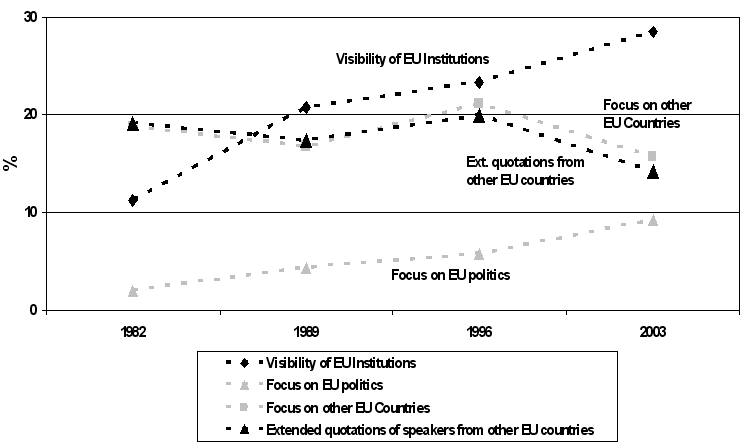
\includegraphics[width=0.95\linewidth]{./SocSci/Wessler.jpg}
%   \mycaption{ xxx )}
    \label{fig:Wessler001}
   \end{center}
\end{figure} \\
Whereas EU institutions and policies are monitored more closely over time in national quality newspapers, and European identity constructions hesitantly enter the public realm in certain instances, the horizontal exchange of opinions between European countries does not increase; national discourse constellations do not become more similar over time. Particular emphasis is placed on case studies of national public debates about Western military interventions, and genetically modified food. Results of Phase I will be published in a number of articles and a monograph with Palgrave Macmillan in 2007. An additional study conducted with IUB students has analyzed online newspapers from ten Eastern and Western European countries with respect to general content characteristics and levels of Europeanization. Apart from work on the European public sphere, Hartmut Wessler has developed a second research line. He completed a pilot study on intercultural aspects of television coverage of the 2003 Iraq war. The project "Different pictures? The Influence of Arab Television Channels on the Image of the Iraq War in Western International Television News Programs" analyzed how Western news channels use material from Arab channels and how they distance themselves from this material at the same time.


\vspace{0.6cm}
\textbf{Funded Projects}\\[-0.25cm]
\begin{enumerate}
\item[$\bullet$]	"The Transnationalization of Public Spheres: The Case of the EU"\newline
funded by the Deutsche Forschungsgemeinschaft as part of the Collaborative Research Center 597 "Transformations of the State"
\end{enumerate}


\vspace{0.6cm}
\textbf{Other Professional Activities}\\[-0.25cm]
\begin{enumerate}
\item[$\bullet$]Deputy member of the board, Collaborative Research Center 597 on "Transformations of the State", funded by the Deutsche Forschungsgemeinschaft
\item[$\bullet$]Reviewer for Volkswagen Foundation, Hannover, \textit{Global Media and Communication, Medien \& Kommunikationswissenschaft, Zeitschrift f�r Medienpsychologie, Journalism: Theory, Practice \& Criticism,} and for Annual conferences of the International Communication Association and the German Communication Association
\end{enumerate}


\vspace{0.6cm}
\textbf{PhD-Students}\\[-0.25cm]

Katharina Kleinen-von K�nigsl�w\newline
\textit{Integration and Segmentation of the National Public Sphere}


\vspace{0.6cm}
\textbf{Research Personnel}\\[-0.25cm]

Michael Br�ggemann\newline
Research Associate in the project "The Transnationalization of Public Spheres: The Case of the EU"\\[-0.15cm]

Stefanie Sifft\newline
Research Associate in the project "The Transnationalization of Public Spheres: The Case of the EU"
